\section{Application to Single-Pixel Imaging}
\label{ch:cs}
\subsection{Introduction}
% SPI definition and main stages
Single-pixel imaging (SPI) is a relatively recent imaging technique that replaces the classic two dimensional sensor array with a single photodetector~\citep{bian2018experimental}. An SPI camera modulates the incoming light from a scene using a light modulator, such as a diffuser~\citep{guo2016multilayer} or a digital micro-mirror device (DMD)~\citep{pittman1995optical, sampsell1993overview}, and focuses the resulting correlated light patterns onto a photodiode. The configuration of the modulator and the recorded intensity of light are then processed to reconstruct an image of the target scene.

% advantages of SPI
SPI owes its popularity to multiple advantages it achieves over traditional imaging approaches that employ 2D sensor arrays. First, since all reflected light is focused onto a single detector, SPI has better sensitivity under dim lighting conditions and enjoys a broader spectral range\citep{Edgar2019}. Second, SPI moves the cost of acquisition and processing from the encoding/compression stage to the decoding/reconstruction stage. For example, a DMD array orients its mirrors to reflect light either towards the detector (+1) or away from it (0). Importantly, these orientations do not depend on the scene that is being acquired to ensure proper reconstruction: \citep{baraniuk2008simple}~showed that DMD patterns can be drawn as independent identically distributed (i.i.d.) samples from a uniform Bernoulli distribution. In contrast, sample-then-compress approaches\citep{skodras2001jpeg} require an expensive projection of multiple single-pixel snapshots onto a chosen basis, such as Fourier or top-K singular vectors, during their encoding step. Doing the heavy-lifting job during decoding is often preferred in applications where sensors have to be small and low-power, whereas decoding happens offline on high-performance computers. The simplicity of encoding keeps the computational requirements of SPI sensors (and thus their price) low, inviting their application in multispectral imaging \citep{bian2016multispectral,li2017efficient}, optical encryption~\citep{chen2013ghost}, remote sensing~\citep{zhao2012ghost}, object tracking~\citep{li2014ghost}, and many other fields~\citep{sun20133d,zhang2010correlated,cheng2009ghost}.

% introducing CS
Compressive Sensing (CS)~\citep{donoho2006compressed, candes2006compressive, baraniuk2014introduction, baraniuk2008simple} emerged in the mid-2000s as an alternative signal acquisition regime to classical Shannon-Nyquist sampling. In the classical regime, a band-limited signal is sampled at $N$ specific points in time (and/or space) so that the signal can be reconstructed from the acquired samples using a simple Sinc interpolation. Compressive sensing, on the other hand, proposes to acquire the signal using a small number of inner products between the signal and general non-adaptive sampling vectors. If the signal to be acquired has a $K$-sparse, or more generally, parsimonious, representation some transform domain, then the signal can be guaranteed to be recovered using as few as $\mathcal{O}(K\log(N/K))$ non-adaptive measurements, which is much smaller than the $N$ samples that are required by sample-then-compress approaches such as JPEG and JPEG-2000~\citep{skodras2001jpeg}. The development of compressive sensing theory and efficient reconstruction algorithms has further promoted the deployment of this technique in SPI~\citep{duarte2008single}.

% Compressive Sensing (CS) is an approach to SPI which assumes that a signal is spare in a certain basis. Under this assumption a small collection of non-adaptive linear measurements can contain enough information for reconstructing the signal~\citep{duarte2008single, candes2006compressive}. Namely, when an original signal made of $N$ pixels has a $K$-sparse representation in a certain basis, the basis coefficients can be recovered using only $\mathcal{O}(K\log(N/K))$ which is much smaller than $N$ required by sample-then-compress approaches such as JPEG and JPEG-2000~\citep{skodras2001jpeg}.

% Recent progress on deep SPI
Since every SPI measurement contains highly-compressed information about the observed frame, one needs to sample a large number of such measurements to allow for faithful reconstruction. Thus, many recent works propose approaches to reduce the number of required samples per frame (SPF). These approaches can be roughly grouped in two buckets: signal-dependent control of the mirrors, and more sophisticated reconstruction techniques. The former ensures that each single-pixel measurement contains as much information as possible by focusing the mirrors on the selected regions of the frame~\citep{zhang2017fast,sun2017russian,xu20181000}. Although highly effective, such approach can not be applied to detectors that do not offer fine-grained control of their mirrors. The latter group focuses on creating more efficient optimization algorithms for the decoding step~\citep{katz2009compressive}. It includes non-iterative algorithms such as differential ghost imaging (DGI) \citep{gong2010method}, as well iterative methods such as total variation (TV)~\citep{suo2016signal} regularized reconstruction. Notably, recent approaches adopted deep learning (DL) for SPI reconstruction and showed that using deep neural networks can dramatically reduce the sampling ratio and offer near-real-time performance \citep{lyu2017deep,higham2018deep,wang2019learning,wang2022single}. However, most of these methods use multiple samples for single-frame reconstruction and do not yield satisfactory reconstruction of multiple sequential frames when the number of samples per frame is small even if the total number of samples collected for the full video sequence is large.

\begin{figure*}
    \centering
    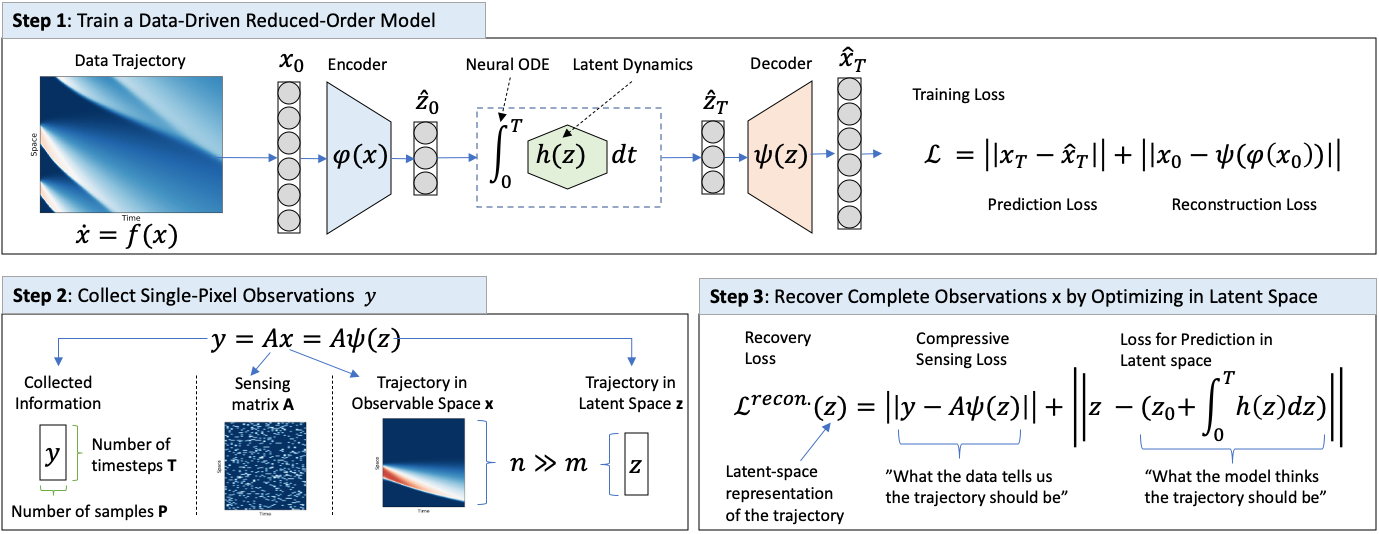
\includegraphics[width=\textwidth]{figures/cs_ga_current.png}
    \caption{\label{fig:cs_abstract}We propose a compressive-sensing algorithm that reconstructs observation by identifying their trajectories in a latent space of a Reduced-Order Model (ROM). The model provides strong inductive bias and reduces data intake requirements for compressive-sensing hardware.}
\end{figure*}

% Our place among CS literature
This work aims to enable high quality reconstruction of videos from a small number of samples per frame. Our approach falls into the second group of decoding-centered approaches which aid SPI reconstruction with deep learning. In particular, we show how a Reduced-Order Model (ROM) can be used to regularize SPI reconstruction of a video of a physical phenomenon, even if all measurements are taken at different moments in time, i.e. when the number of samples per frame is one. We achieve that by pre-training a ROM to compress simulations into a latent space and calculate the system's evolution within the latent space using neural ordinary differential equations (Neural ODEs). The reconstruction procedure minimizes the measurement mismatch between the samples recorded by the SPI detector and the synthesized measurements obtained by sampling the reconstructed trajectory using a measurement operator $A$. Effectively, we solve an ODE-regularized SPI reconstruction in an efficient way using the adjoint-sensitivity method to obtain the necessary derivatives~\citep{chen2018neuralode}. Such ODE-based regularization provides a strong signal prior and allows for the reduction in the number of samples per frame required for successful reconstruction below the requirements of current state-of-the-art methods. We introduce the methodology in Section~\ref{sec:cs_methods} and study its performance on three examples: Burger's equation, Kolmogorov flow, and methane leaks videos from GasVid dataset \citep{wang2020machine}.

\subsection{Methods}
\label{sec:cs_methods}
\paragraph{Single-Pixel Imaging} 

\begin{figure}
\centering
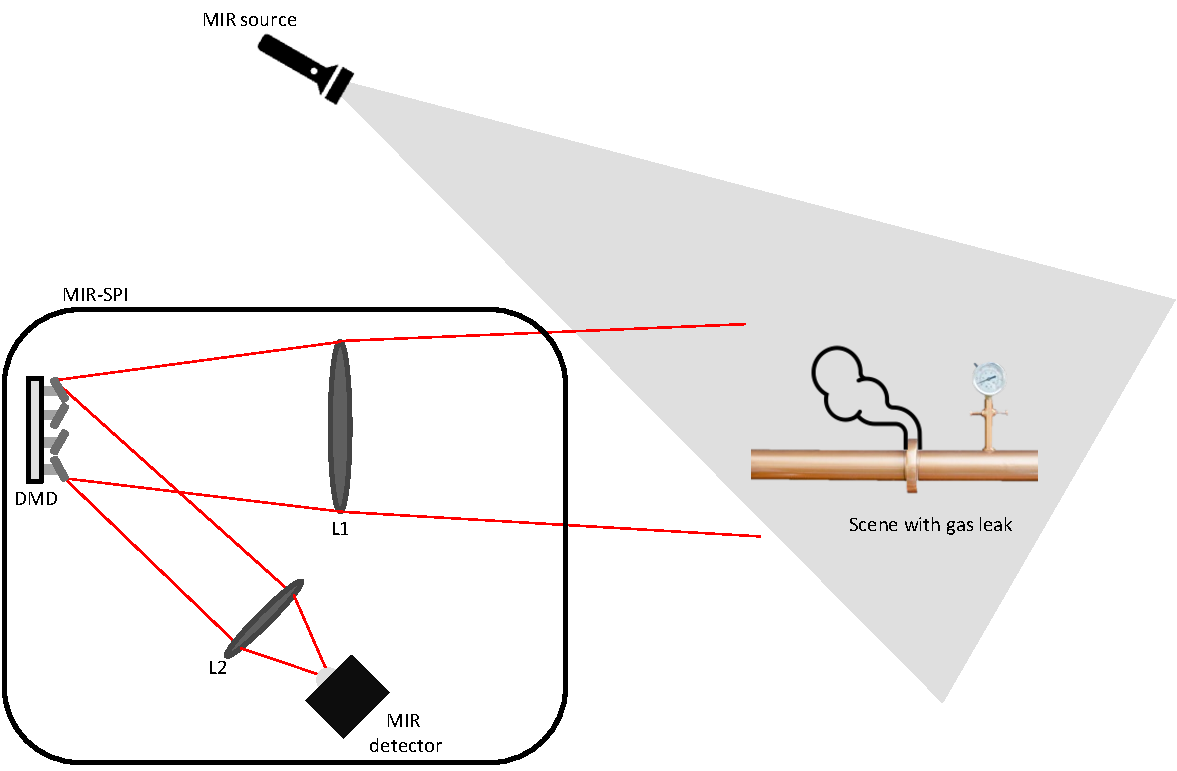
\includegraphics[width = 0.5\textwidth]{figures/SPI_setup.pdf}
\caption{A schematics for Single-Pixel Imaging setup with Digital Micro-mirror Device (DMD) \label{fig:SPI}}
\end{figure}

Let $x(t) \in \XX \subseteq \mathbb{R}^n$ be a representation of a high-dimensional spatio-temporal system, e.g. a video recording of a scene that we observe. In many applications we can not record $x(t)$ in real time due, for example, to monetary costs that a necessary equipment would impose. Instead, we collect records from $p$ detectors, where each detector provides a linear combination of coordinates of $x(t)$ at a time:
\begin{equation}
    \label{eq:cs_definition}
    y(t_i) = A_i x(t_i), \quad A_i \in \mathbb{R}^{p\times n}, \quad t_i \in [0, T],\quad i \in 0 \dots K
\end{equation}

In particular, we consider a single pixel camera setup where for every time instance $t_i$, a vector of $p$ acquisitions $y_i \in \mathbb{R}^p$ are obtained by a high sampling rate photo-detector using the projection matrix $A_i$. The rows of the matrix $A_i$ correspond to a binary mask pattern that can be encoded using a digital micro-mirror device (DMD, ~\citep{pittman1995optical, sampsell1993overview}). In this setup, the mirrors of the DMD array represent pixels of the future reconstructed image and slopes of the mirrors represent the weights. The light from a scene lands on a DMD which slopes its every mirror to reflect light either towards the detector (+1) or away from it (0) according to a uniform Bernoulli variable. Next, the (+1) pixels go through a double-convex lens that focuses it on a signal photon detector. Finally, the detector integrates the signal and provides the final observation as its output voltage, which is later digitized by an A/D converter~\citep{duarte2008single}. The slopes of each mirror are also recorded in the detector's memory. Figure~\ref{fig:SPI} illustrates an example of the single pixel imaging setup where a gas plume is imaged using a DMD array and a medium infra-red (MIR) photo-detector. 

Multiple techniques attempt reconstruct $x(t)$ directly by inverting the relation~\ref{eq:cs_definition} under mild regularity priors; examples include Differential Ghost Imaging (DGI, \citep{ferri2010differential}), Total Variation Regularization (TVR, \citep{bian2018experimental}), and Fourier Domain Regularization (FDRI, \citep{pastuszczak2021differential}).  Alternatively, one can recover $x(t)$ by recovering its projection $z(t) \in \ZZ \subseteq \mathbb{R}^m$ on a low-dimensional manifold ($m \ll n$). Namely, if we know  an invertible mapping $\psi(z): \ZZ \to \XX$ then we can trade a problem of recovery of a high-dimensional vector $x$ using $p$ linear observations to recovery of a low-dimensional vector $z$ using $p$ non-linear observations:

\begin{equation}
    \label{eq:cs_with_ae}
    y(t) = A_t\psi(z(t))
\end{equation}


 We call the space $\XX$ an observable space, $\ZZ$ a latent space, and the mapping $\psi(z)$ a true decoder. Often $\psi(z)$ is not known, in which case an approximation $\psi_\theta(z)$ is trained using a dataset of collected images $\{x_1, \dots, x_N\}$, where $\theta$ denotes the parameters of the model, e. g. the weights of an autoencoder network. However, if $y(t)$ is insufficient for a unique reconstruction of $x(t)$ then it will remain insufficient for reconstructing $z(t)$. Thus, introducing additional structural sparsity or priors is required to make the autoencoder-based reconstruction work, such as joint training of the sampling matrices and the decoder by \citep{wang2022single}. In this work we take a different route and supplement the encoder $\psi(z)$ with knowledge of the dynamics of $z(t)$ on the manifold over time. 

\paragraph{Reduced-Order Model with Non-Linear Latent Dynamics}
Let $x(t)$ be modelled as an autonomous dynamical system on a finite space $\XX \subseteq \mathbb{R}^n$

\begin{equation}
    \label{eq:cs_generic_stationary_ode}
        \ddt\bd{x}(t) = \bd{f}(\bd{x}(t))
\end{equation}

In real-world applications it is often expensive to use the relationship~(\ref{eq:generic_stationary_ode}) for predicting the behaviour of the system even when $f(x)$ is known because $x(t)$ can be very high-dimensional. For example, if $x(t)$ is a flow of 2D liquid then $\bd{f}(x)$ may be a discretization of Navier-Stokes equations, in which case running a simulation~\ref{eq:cs_generic_stationary_ode} may take months on a cluster. However, a variety of works provided both theoretical (\citep{holmes2012turbulence}) and practical (\citep{noack2011reduced,chen2021discovering}) evidence that many physical systems evolve on a lower-dimensional manifold $\ZZ$. In that space, the dynamics evolve according to a (generally unknown) function  $\bd{h}(\bd{z})$:

\begin{equation}
        \ddt\bd{z}(t) = \bd{h}(\bd{z}(t))
\end{equation}

 Thus, one can predict the dynamics of the system $\bd{x}$ at a future time $T$ by projecting the initial condition $\bd{x}(0)$ into the latent space, performing an integration there, and mapping the resulting trajectory back to the observable space:
\begin{equation}
\label{eq:cs_integration_in_latent_space}
\begin{split}
    \bd{z}(0) & = \psi^{-1}(\bd{x}(0)) \\
    \bd{z}(T) & = \bd{z}(0) + \int_{0}^T\bd{h}(\bd{z}(t))dt \\
    \bd{x}(T) & = \psi(\bd{z}(T))
\end{split}
\end{equation}

When $m \ll n$ we refer to the triplet $(\psi, \psi^{-1}, \bd{h})$ as a Reduced-Order Model (ROM) of $\bd{f}$. It is often the case that for a given system $\bd{f}$ there exists no ROM $(\psi, \psi^{-1}, \bd{h})$ such that the relation~(\ref{eq:cs_integration_in_latent_space}) holds exactly. In this case, we seek an \textit{approximation} ROM $(\psi_{\theta^*}, \phi_{\theta^*}, h_{\theta^*})$ that minimizes the difference between the data $x(t)$ and the prediction $\hat{x}(t)$ over a chosen class of models $(\psi_\theta, \phi_\theta, h_\theta)$ parameterized by $\theta$.


\paragraph{Architecture} In this work we model $\psi$, $\psi^{-1}$, and $\bd{h}$ with neural networks $\psi_\theta$, $\phi_\theta$, and $h_\theta$, respectively. Specifically, the pair ($\psi$, $\psi^{-1}$) is modelled with an auto-encoder $(\psi_\theta, \phi_\theta)$, and $\bd{h}$ is modelled with a fully-connected network $h_\theta$, as illustrated in the first frame of Figure~\ref{fig:cs_abstract}. All considered models share this architecture; however, the exact architectures of the functions $\psi_\theta$, $\phi_\theta$, and $h_\theta$ are problem-dependent and discussed more closely in the related sections. 

\paragraph{Training Loss} Similar to prior works by \citep{takeishi2017learning,morton2019deep,gin2021deep}, we define a \textit{training loss} $\LL$ as a sum of reconstruction and prediction losses. The former ensures that $\phi_\theta$ and $\psi_\theta$ are inverse mappings of each other, whereas the latter matches the model's predictions to the available data. Formally, for a given set of trajectories $\bd{x}_i$, $i \in [1 \dots N]$, where each trajectory $\bd{x}_i \in \mathbb{R}^{n \times K}$ is a set of $p$ snapshots of the system for each time-step, for $K$ time-steps, $t_i$, $i \in [0, \dots, K]$, the loss function $\LL^{data}_\theta$ is defined as:

\begin{align}
    \label{eq:cs_loss_data_driven}
    \LL(\theta) & = \sum_{i = 1}^N \left[\sum_{j=0}^K\left\|\bd{x_i}(t_j) - \psi_\theta(\phi_\theta(\bd{x_i}(t_j)))\right\|^2\right. + \\
     & + \left.\sum_{j=1}^K \left\|\psi_\theta\left(\phi_\theta(\bd{x_i}(t_0)) + \int_{t_0}^{t_j}h(z(t))dt\right) - \bd{x_i}(t_j)\right\|^2 \right]
\end{align}
where $\sigma$ is the standard deviation of the observation noise.

To obtain a ROM $(\psi_{\theta^*}, \phi_{\theta^*}, h_{\theta^*})$, we minimize the loss above. We note that each trajectory $\bd{x}_i$ may be captured over its own time-frame and use a distinct, possibly non-uniform, step-size, in which case the loss function should be modified accordingly\footnote{The implementation is affected only in evaluating the integral in~(\ref{eq:cs_loss_data_driven}). This part is handled by \texttt{torchdiffeq}~\citep{chen2018neural} library, which supports non-uniform time-frames within a batch}. To simplify the notation without loss of generality, in the rest of the work we assume that all trajectories were recorded over the same time-frame with an equal and uniform step-size. 

\paragraph{Recovery Loss} 
We use the ROM $(\psi_{\theta^*}, \phi_{\theta^*}, h_{\theta^*})$ above to regularize the latent-space dynamics of the single-pixel imaging reconstructions. Namely, we obtain the reconstruction $x^* = \psi(z^*)$ by minimizing the following loss with respect to $z = [z_0, \dots, z_K] \in \mathbb{R}^{m \times K}$.

\begin{equation}
    \label{eq:cs_reconstruction_loss}
     \LL_{\theta^*}^{recon}(z) = \sum_{j=0}^K  \left\|y_j - A\psi_{\theta^*}(z_j)\right\|_2^2 + \lambda \left\|z_0
     + \int_{t_0}^{t_j}h_{\theta^*}(z)dz - z_j\right\|_2^2
\end{equation}

where the parameter $\lambda$ controls the degree on which the compressing sensing algorithm relies on the latent dynamics $h_{\theta^*}$ during the signal reconstruction phase. We minimize the loss~\ref{eq:cs_reconstruction_loss} using a gradient-based technique, with the gradients obtained using automatic differentiation frameworks. 

\subsection{Experiments}

\subsubsection{Burger's Equation}
We study the performance of our framework on Burger's equation with $[-\pi, \pi]$-periodic boundary conditions:

\begin{equation}
\begin{split}
\label{eq:cs_burgers_equation}
    & u_t  + uu_x = \nu u_{xx} \\
    & u(-\pi, t) = u(\pi, t),\quad \forall t \in [0, T]
\end{split}
\end{equation}
where $u_t$, $u_x$, and $u_{xx}$ represent partial derivatives in time, the first, and second spatial derivatives, respectively. 

\paragraph{ROM Training} To obtain train dataset for the ROM we replicate the experimental setup from Section~\ref{sec:burger_eqn}. Namely, we generate 1024 trajectories on a discretized spacial domain $[-\pi,\,\pi]$ with 128 grid-points. To generate a diverse set of initial conditions we sum the first 10 harmonic terms with random coefficients:
\begin{equation}
    \label{eq:burger_initial_condition_sine}
    \begin{split}
        u(x, 0) = & \frac{1}{10}\sum_{k = 1}^{10} a_k\cos(kx) + b_k\sin((k+1)x)\\ & a_k, b_k \sim \mathcal{N}(0, 1)
    \end{split}
\end{equation}
 We solve Equation~\ref{eq:cs_burgers_equation} for $t \in [0, 2]$ with $\Delta t = 0.1$ using a spectral solver by~\citep{trefethen2000spectral}. 

\begin{figure}[t]
    \centering
    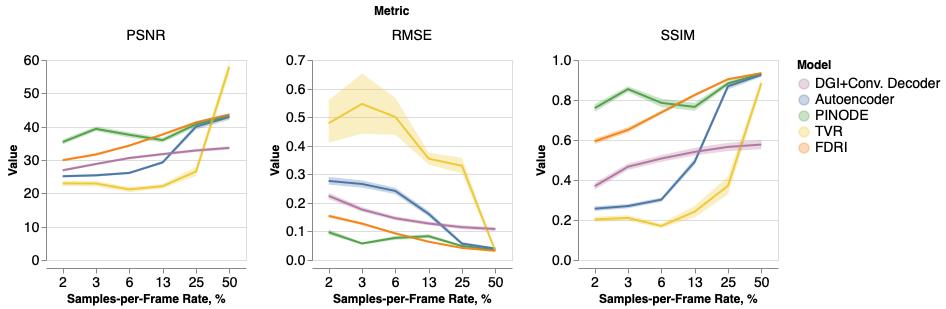
\includegraphics[width=\textwidth]{figures/cs_burgers_psnr.png}
    \caption{\label{fig:cs_burgers_spf} Median PSNR, RMSE, and SSIM with 25-27th percentile intervals over different number of samples per frame taken.}
\end{figure}

\begin{figure}[t]
    \centering
    	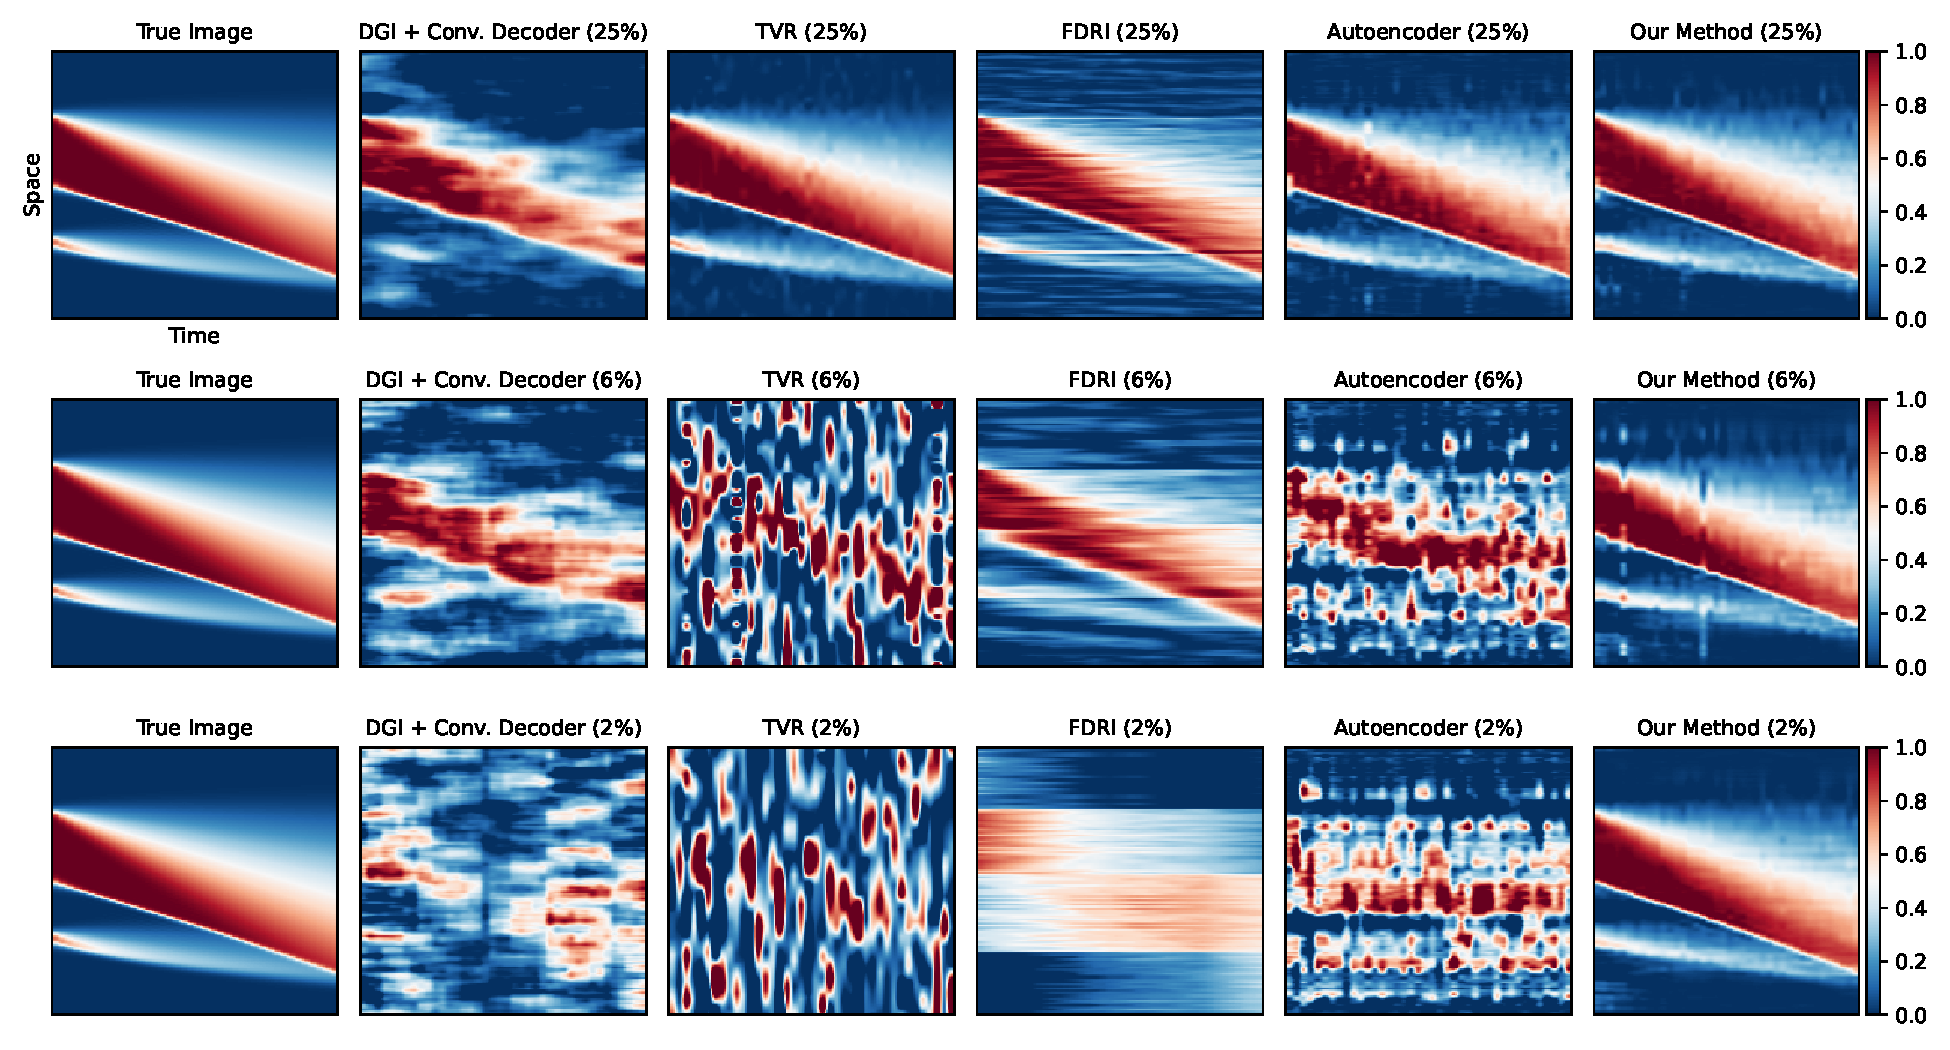
\includegraphics[width=\textwidth]{figures/cs_burgers_comparison_all.pdf}
    \caption{\label{fig:cs_burgers_example_large_spf} Example reconstruction of a trajectory of Burgers' equation for three SPF rates: 25\%, 6\%, and 2\%. All algorithms complete the reconstruction faithfully when SPF is large. However, all algorithms except our proposed method, fail to recover the image due to the insufficient SPF rate ($2/128 \lesssim$ 2\%). In contrast, our proposed method achieves nearly the same reconstruction quality as in with SPF rate of 25\%.}
\end{figure}

\paragraph{Recovery}
For the SPI Recovery phase, we generate 128 trajectories with ``bump'' initial conditions -- a smooth approximation of a bump with two opposing steeply-curved sigmoids:

\begin{equation}
    \label{eq:burger_initial_condition_bumps}
    u(x, 0) = \frac{1}{1 + exp(-k(x-a))} - \frac{1}{1 + exp(-k(x-b))}
\end{equation}
where $a < b$ are sampled uniformly in $[-\pi, \pi]$ and $k = 20$. We choose this shape to ensure that the training and sensing trajectories are sufficiently different. We choose sensing matrices $A_t$ to be binary (0-1) matrices with each row having 64 non-zero components out of 128 sampled uniformly.



We compare our approach (PINODE) with four alternatives: an Autoencoder-enhanced variation of Digital Ghost Imaging, \citep{ferri2010differential,gong2010method}(DGI+Conv. Decoder, \citep{wang2022single}) Total Variation Regularization  (TVR, \citep{bian2018experimental}), Fourier Domain Regularization (FDRI, \citep{czajkowski2018real}), and an approach which uses an autoencoder (AE, \citep{bora2017compressed}). We measure reconstruction accuracy with three commonly-used metrics: the residual mean-squared error (RMSE), the peak signal-to-noise ratio (PSNR), and the structural similarity index measure (SSIM). We evaluate both metrics for Burger's trajectories as 2D-images in spatial and in temporal domains. 

For two 2D images $a$ and $b$, PSNR is defined as the log-ratio of the maximal value from the true image:

\[
	\text{PSNR}(a, b) = 20\log\left(\frac{\max_{i,j}(|a[i,j]|)}{\|a - b\|_2}\right)
\]

SSIM is defined as a product of relative luminance $l(a,b)$, contrast $c(a,b)$, and structure $s(x,y)$:

\[
	\text{SSIM}(a, b) = l(a,b) \cdot c(a,b) \cdot s(a,b) = \left(\frac{2\mu_a\mu_b + c_1}{\mu_a^2 + \mu_b^2 + c_1}\right) \cdot \left(\frac{2\sigma_a\sigma_b + c_2}{\sigma_a^2 + \sigma_b^2 + c_2} \right) \cdot \left(\frac{\sigma_{ab} + c_2/2}{\sigma_a \sigma_b + c_2/2}\right)
\]
where, for a picture $x$, $\mu_x$ is the pixel sample mean, $\sigma_x$ is the standard deviation,  and $c_i$ are the constants which stabilize the division when the denominator approaches 0. Typically, $c_i$ are set to be proportional to the square of the dynamic range of the pixel values, e.g.  $c_i = (k_i*2^{\text{bits per pixel}} - 1)^2$, with $k_1 = 0.01$ and $k_2 = 0.03$ being default choices.
Finally, RMSE is defined as the mean residual squares for every state, averaged over the temporal axis:

\[
	\text{RMSE}(a,b) = \|a - b\|_F.
\] 

\paragraph{Results} The results are presented in Figure~\ref{fig:cs_burgers_spf}. We plot median PSNR, RMSE, and SSIM over different number of samples per frame taken. We see that PINODE achieves 70\% higher peak signal-to-noise-ratio (PSNR) and 4 times higher structural similarity index measure (SSIM)  relative other algorithms when SPF is low. We also see that the DGI and TVR approaches do not reconstruct images faithfully until SPF approaches the number of pixels in a snapshot; Figure~\ref{fig:cs_burgers_example_large_spf} provides an example of high-SPF reconstruction. In contrast, PINODE is able to reconstruct most trajectories with high accuracy using a very small number of samples per frame e.g. two samples. It happens because the reduced-order model of PINODE serves as a strong prior: the model reconstructs the trajectory as a whole instead of reconstructing every snapshot separately, as all other algorithms do in this comparison. It allows PINODE to borrow strength across snapshots, even when SPF per each snapshot is small.


\subsubsection{Kolmogorov Flow}

\label{sec:kolmogorov_flow}
We study the performance of our framework on Kolmogorov-like flow first-described by~\citep{dovzhenko1981generation} and later analyzed by \citep{tithof2017bifurcations,suri2017forecasting}. The following equation describes the behavior of a 2D velocity field $\bd{u}(x, y, t)$:


\begin{align}
\label{eq:kolmogorov_flow_definition}
	& \partial_t \bd{u} + \bd{u} \cdot \nabla \bd{u} = -\nabla p + \nu\nabla^2\bd{u} + f \\
	& \nabla \cdot \bd{u} = 0
\end{align}

\begin{figure}[t]
    \centering
    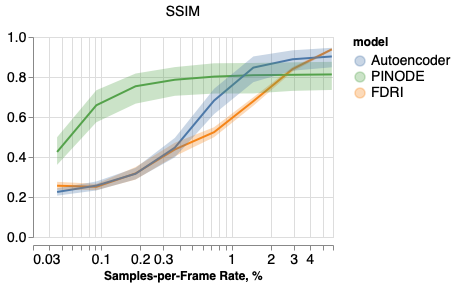
\includegraphics[width=0.5\textwidth]{figures/cs_kolm_aggregate_all.png}
    \caption{Caption}
    \label{fig:cs_kolm_agg}
\end{figure}

where $p$ is a 2D pressure field, $f = \alpha\sin(ky)x$ represents the driving force with amplitude $A$ and wavenumber $k$, and $\nu = 1/\text{Re}$ is the non-dimensional viscosity equal to inverse of the Reynolds number. In all our experiments, $k = 4$ and $\text{Re} = 40$; we chose this setup to match the one from~\citep{wan2018data}, who identified that this combination of hyper-parameters leads to the occurrence of extreme instability events, making the prediction of such flow truly challenging. 

To train a ROM which predicts $u(x, y, t)$ we generate 8192 data trajectories as solutions of~\eqref{eq:kolmogorov_flow_definition} using a spectral solver\footnote{\href{https://github.com/zhong1wan/data-assisted/blob/master/Kolmogorov/kol2d_odd.py}{https://github.com/zhong1wan/data-assisted/blob/master/Kolmogorov/kol2d\_odd.py}} from~\citep{wan2018data}. Each solution was simulated from t=0 to t=100 to get past the transient regime and then recorded from t=100 to t=110, with the time-step $dt=0.5$. As in Section~\ref{sec:method}, the ROM consists of an encoder $\phi(u)$, a decoder $\psi(z)$, and the latent dynamics $h(z)$. It was trained by minimizing the data-driven loss~\eqref{eq:loss_data_driven} until the prediction RMSE on a holdout set stopped improving, which took about 60 epochs. 

\begin{figure}[t]
	\centering
	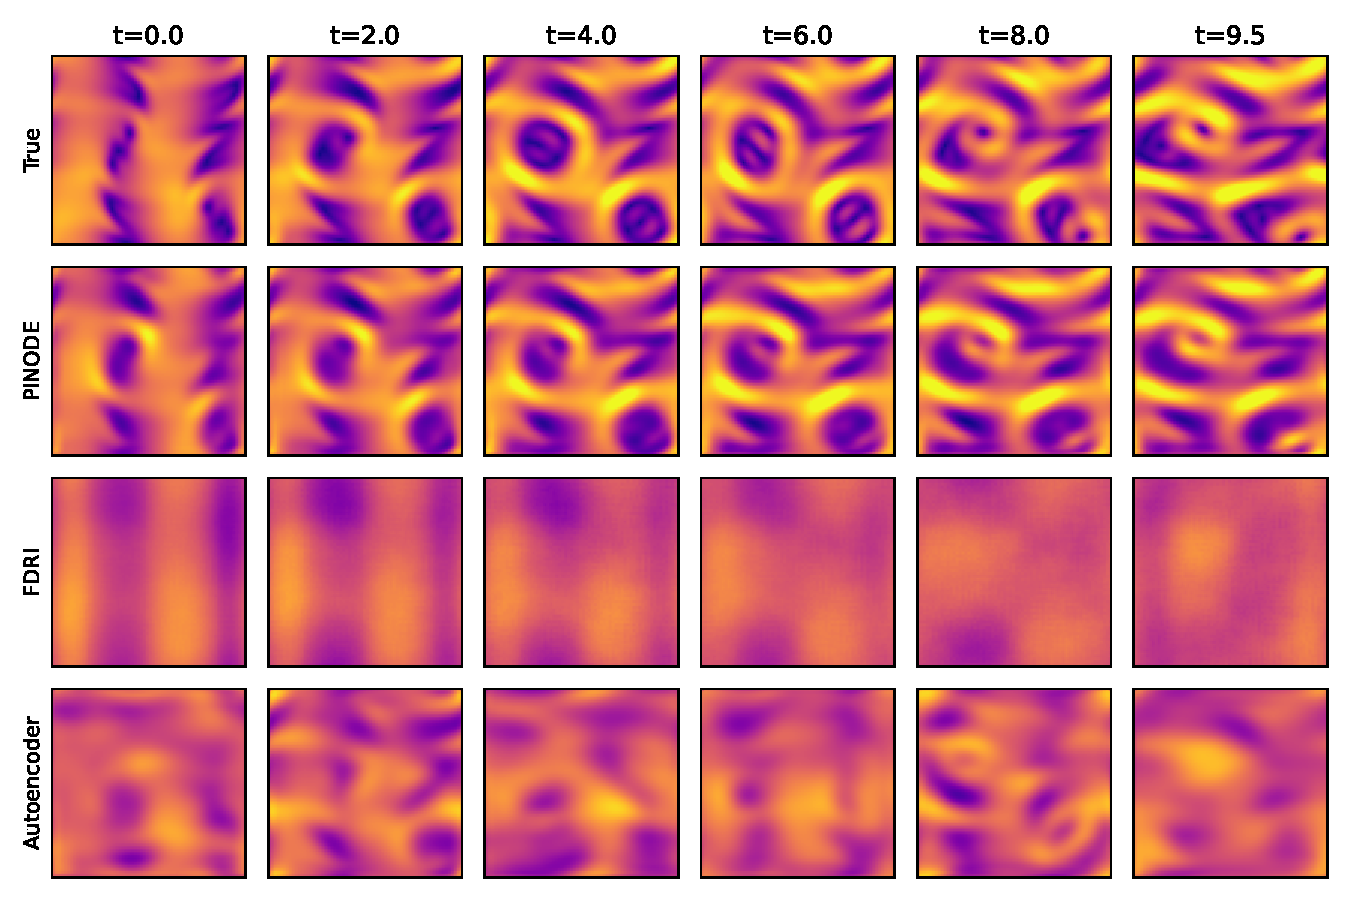
\includegraphics[width=\textwidth]{figures/cs_kolm_example.pdf}
	\caption{\label{fig:kolmogorov_example} An example of a reconstruction of Kolmogorov with three different methods using 8 samples per frame of $66\times 66$ pixels, an SPF rate of 0.18\%.}
\end{figure}

A sample result is displayed on Figure~\ref{fig:kolmogorov_example}. The columns represent different timesteps. The first row represents the true flow, the next three rows represent our method, FDRI, and Autoencoder methods respectively. We acquire 8 samples per frame where each frame consists of $66\times 66=4356$ pixels, which yields a sampling-per-frame rate of 0.18\%. We observe that the reconstruction faithfully recovered the signal whereas two other algorithms fail to recover the image. The aggregated results on Figure~\ref{fig:cs_kolm_agg} show that other methods require more than 2\% SPF rate for a faithful recovery of the signal, whereas our method can provide a decent reconstruction with SPF as low as 0.18\%, a difference of one order of magnitude in required data intake.

\subsubsection{Methane Leaks Data}
In this section we use our technique to reconstruct videos of gas leaks using observations from a single-pixel camera. We use a subset of GasVid dataset by~\citep{wang2020machine} which consists of recordings of a methane gas leaks. 10 videos 10 to 20 seconds each. We split them into 1-second-long intervals, where each interval contains 10 steps: $T = 1$ sec., $dt = 0.1$ sec. Next, we remove backgrounds from each video using Gaussian Mixture-based Background/Foreground Segmentation (MOG2) algorithm by~\citep{zivkovic2006efficient,zivkovic2004improved} implemented in OpenCV library~(\citep{opencv_library}). Finally, we split all intervals into four non-overlapping batches: train (390), dev (50), test (49), and SPI (2). We use the first three to train, fine-tune, and select a final ROM respectively, and then we use the fourth batch for SPI reconstruction. We use the same architecture of ROM as in Section~\ref{sec:kolmogorov_flow}. At the recovery step we sample 512 single-pixel observations per each $240 \times 320$ video frame; it corresponds to SPF ratio of $0.66\%$ (2/3 of one percent).

\begin{figure}[t]
	\centering
	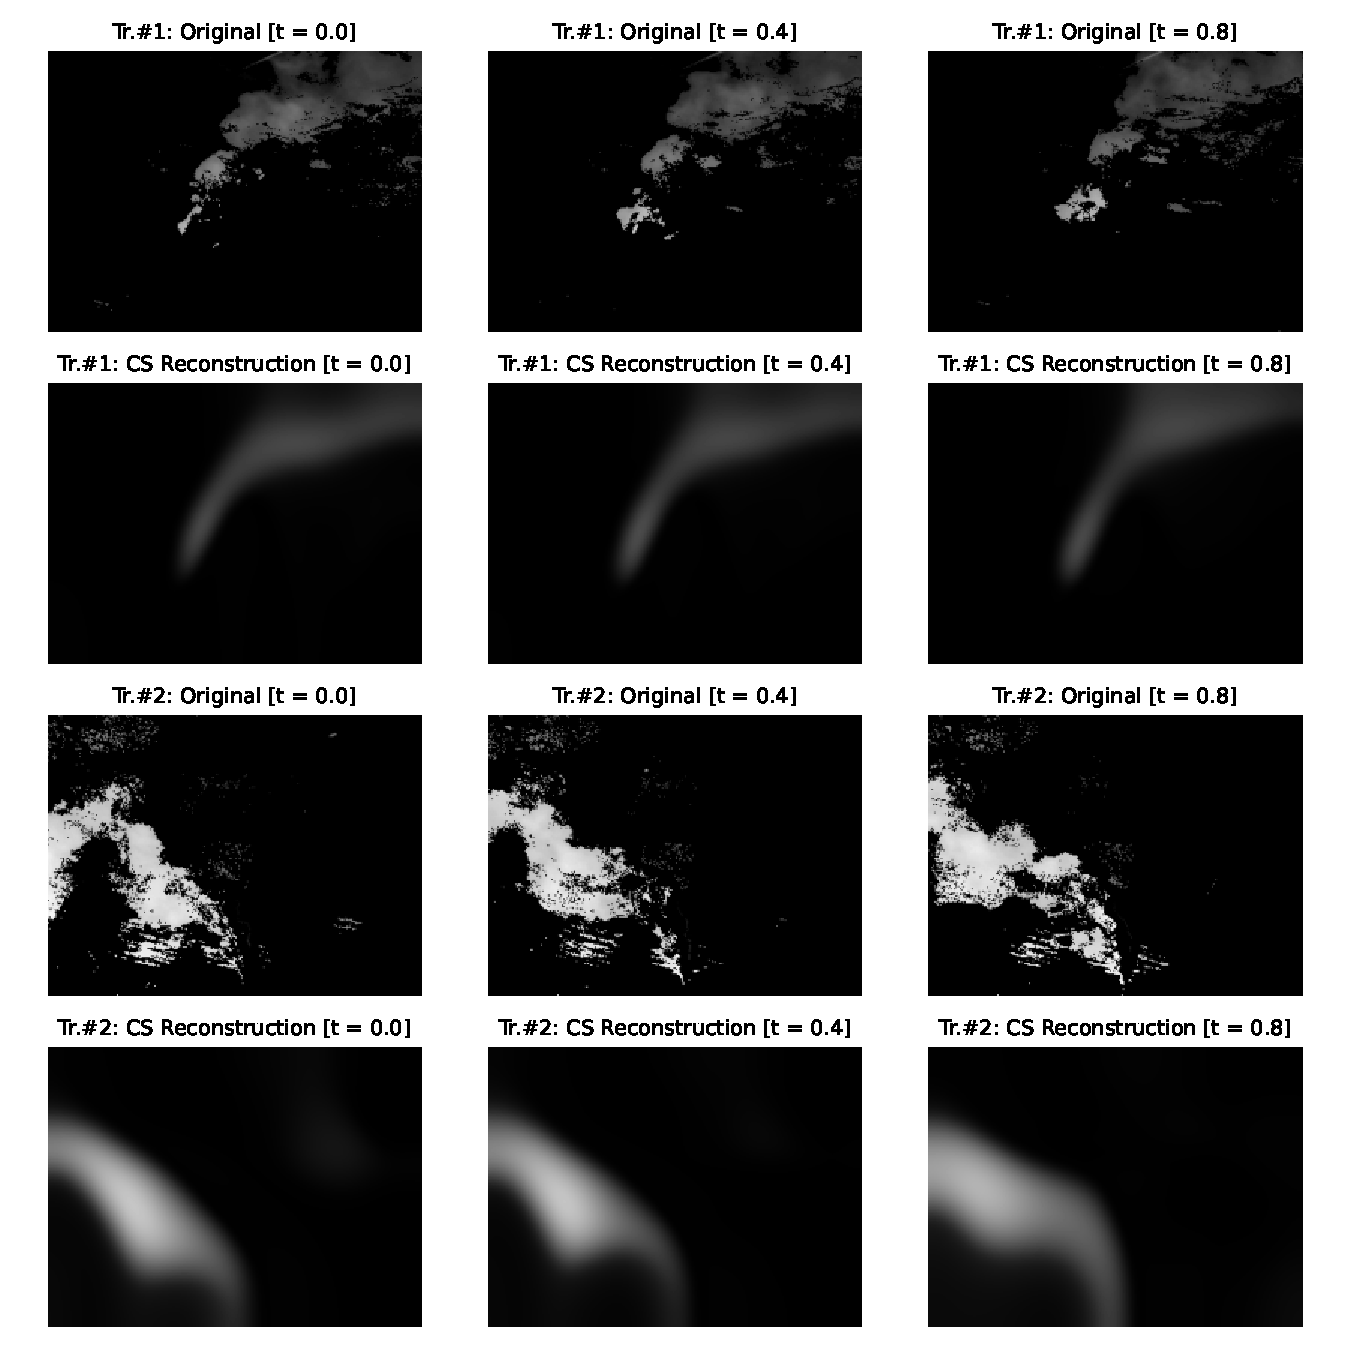
\includegraphics[width=\textwidth]{figures/cs_gas_examples.pdf}
	\caption{\label{fig:cs_gas_examples} Results of a Single-Pixel Imaging reconstruction for Methane Leaks Data using Equation~\ref{eq:cs_reconstruction_loss}. We trained a ROM (Equation~\ref{eq:cs_loss_data_driven}) using 489 training trajectories, each having 10 video frames 0.1 seconds apart. This dataset is a subset of GasVid dataset by \citep{wang2020machine}}.
\end{figure}

The example reconstructions are presented on Figure~\ref{fig:cs_gas_examples}. We see that the algorithm was able to faithfully reconstruct the trajectories. Although it was unable to capture the details of turbulent flows, it was able to predict the altitude, the direction, and the spread of the plumes correctly, which are the most important aspects for practical applications in real-world gas monitoring applications. 

We note the threefold difficulty of the task. First, the background subtraction struggles to separate grey smoke from a dynamic grey background, which leads to fantom clouds of smoke in processed data. Second, the amount of training data (3900 frames) is extremely small for training a large convolutional ROM. For example, \citep{wang2020machine} used the same dataset for training a simpler classification network (leak/non-leak) using ~11000 frames. Finally, an SPF of 0.66\% is vastly insufficient for frame-by-frame reconstruction, as most state-of-the-art methods require ~5-10\% SPF, depending on the nature of the picture (	\citep{wang2022single}). Thus, the inductive bias of the ROM becomes a crucial component for a successful video reconstruction.


\subsection{Discussion} 
In this work, we demonstrated how a collocation-point-based technique can improve the performance of an emerging class of continuous-time physics-informed neural-network-based reduced-order models. First, we demonstrated that the incorporation of collocation points in training data can ``cover the gaps'' in training trajectories and inform the model about underrepresented basins of attraction. Such an approach alleviates the demand for large volumes of data that is common in network-based models. Reducing the amount of data required to faithfully reconstruct a signal is extremely valuable in applications where data is scarce and expensive. Second, the physics-informed loss may work as a safeguard, providing a noise-free source of underlying dynamics.
Third, collocation points can stabilize the model's long-term predictions, allowing for accurate forecasting far beyond the training time horizon. Finally, together with using neural-ODE-based nonlinear latent dynamics, adding physics-informed loss leads to the discovery of more compact latent space representations that also yield more accurate models. Simultaneous stability and compactness is especially important if one aims to use models with SPI and control algorithms. With respect to the computational complexity, we note that adding $Tk$ collocation points to the training imposes less of a computational burden than adding $k$ data trajectories, because, unlike data trajectories, collocation points do not require computing integrals forward in time. The last section served to illustrate how PINODE models that were developed in Section~\ref{sec:method} can help in applied modeling. In particular, we showed how one can employ a PINODE model for compressive-sensing purposes. We illustrated its performance on two examples: Burger's equation and Kolmogorov flow. In these cases, it is clear that PINODE can serve as a powerful regularizer and allow users to go significantly below the limits of the Nyquist sampling theorem. 

One clear limitation of the current work is that the choice of an efficient collocation family is a design decision that a practitioner makes. We believe that such decisions can be automated by adopting existing approaches from classic works on numerical approximations of PDEs, which we leave for future research. Another automation that prompts future research is deriving efficient ways of sampling collocation points, possibly via applying modern adaptive learning techniques (\citep{subramanian2022adaptive}). Finally, although Section~\ref{sec:burger_noise} provides some rationale for why one may expect robustness of hybrid models under noise, we believe that a more rigorous analysis is possible, particularly one that provides conditions under which such robustness is guaranteed. 
